% Options for packages loaded elsewhere
\PassOptionsToPackage{unicode}{hyperref}
\PassOptionsToPackage{hyphens}{url}
%
\documentclass[
]{article}
\usepackage{amsmath,amssymb}
\usepackage{iftex}
\ifPDFTeX
  \usepackage[T1]{fontenc}
  \usepackage[utf8]{inputenc}
  \usepackage{textcomp} % provide euro and other symbols
\else % if luatex or xetex
  \usepackage{unicode-math} % this also loads fontspec
  \defaultfontfeatures{Scale=MatchLowercase}
  \defaultfontfeatures[\rmfamily]{Ligatures=TeX,Scale=1}
\fi
\usepackage{lmodern}
\ifPDFTeX\else
  % xetex/luatex font selection
\fi
% Use upquote if available, for straight quotes in verbatim environments
\IfFileExists{upquote.sty}{\usepackage{upquote}}{}
\IfFileExists{microtype.sty}{% use microtype if available
  \usepackage[]{microtype}
  \UseMicrotypeSet[protrusion]{basicmath} % disable protrusion for tt fonts
}{}
\makeatletter
\@ifundefined{KOMAClassName}{% if non-KOMA class
  \IfFileExists{parskip.sty}{%
    \usepackage{parskip}
  }{% else
    \setlength{\parindent}{0pt}
    \setlength{\parskip}{6pt plus 2pt minus 1pt}}
}{% if KOMA class
  \KOMAoptions{parskip=half}}
\makeatother
\usepackage{xcolor}
\usepackage[margin=1in]{geometry}
\usepackage{longtable,booktabs,array}
\usepackage{calc} % for calculating minipage widths
% Correct order of tables after \paragraph or \subparagraph
\usepackage{etoolbox}
\makeatletter
\patchcmd\longtable{\par}{\if@noskipsec\mbox{}\fi\par}{}{}
\makeatother
% Allow footnotes in longtable head/foot
\IfFileExists{footnotehyper.sty}{\usepackage{footnotehyper}}{\usepackage{footnote}}
\makesavenoteenv{longtable}
\usepackage{graphicx}
\makeatletter
\def\maxwidth{\ifdim\Gin@nat@width>\linewidth\linewidth\else\Gin@nat@width\fi}
\def\maxheight{\ifdim\Gin@nat@height>\textheight\textheight\else\Gin@nat@height\fi}
\makeatother
% Scale images if necessary, so that they will not overflow the page
% margins by default, and it is still possible to overwrite the defaults
% using explicit options in \includegraphics[width, height, ...]{}
\setkeys{Gin}{width=\maxwidth,height=\maxheight,keepaspectratio}
% Set default figure placement to htbp
\makeatletter
\def\fps@figure{htbp}
\makeatother
\setlength{\emergencystretch}{3em} % prevent overfull lines
\providecommand{\tightlist}{%
  \setlength{\itemsep}{0pt}\setlength{\parskip}{0pt}}
\setcounter{secnumdepth}{-\maxdimen} % remove section numbering
\ifLuaTeX
  \usepackage{selnolig}  % disable illegal ligatures
\fi
\IfFileExists{bookmark.sty}{\usepackage{bookmark}}{\usepackage{hyperref}}
\IfFileExists{xurl.sty}{\usepackage{xurl}}{} % add URL line breaks if available
\urlstyle{same}
\hypersetup{
  pdftitle={Bitacora Tesis},
  pdfauthor={Erik Martinez},
  hidelinks,
  pdfcreator={LaTeX via pandoc}}

\title{Bitacora Tesis}
\author{Erik Martinez}
\date{2024-05-15}

\begin{document}
\maketitle

\hypertarget{primer-modelo}{%
\section{Primer modelo}\label{primer-modelo}}

1.-\[ d{T_{L}} = \alpha_{1} T_{L} - \alpha_{2} T_{L}M_{\phi} - \alpha_{3}T_{L}C_{N} - \mu T_{L} \]

2.-\[ dT_{i} = \alpha_{2}T_{L}M_{\phi} + \alpha_{3}T_{L}C_{N} - \alpha_{4}M_{\phi}iT_{i}-\alpha_{5}M_{\phi}iCD8 - \alpha_{6}C_{i}CD8 - \mu T_{i} + \alpha_{9}T_{i} \]

3.-\[ dM_{\phi} = \alpha_{7}M_{\phi} - \alpha_{2}T_{L}M_{\phi} - \mu M_{\phi} \]

4-.\[ dM_{\phi}i = \alpha_{2}T_{L}M_{\phi} - \alpha_{5}M_{\phi}iCD8 -\mu M_{\phi}i \]

5.-\[ dC_{N}= \alpha_{8}C_{N} - \alpha_{3}T_{L}C_{N} - \mu C_{N} \]

6.-\[ dC_{i} = \alpha_{3}T_{L}C_{N} - \alpha_{6}C_{i}CD8 - \mu C_{i} \]

7.- \[ dCD8 = \alpha_{10} CD8 - \mu CD8 \]

\hypertarget{explicacion}{%
\subsection{Explicacion}\label{explicacion}}

\hypertarget{primera.-parasitos-libres}{%
\subsubsection{Primera. Parasitos
libres}\label{primera.-parasitos-libres}}

\[ +\alpha_{1} T_{L}  \] hace referencia a la entrada de protozoarios a
el huesped o al sistema. Sin embargo no debe de multiplicarse por que no
depende de los parasitos iniciales que haya o no dentro del huesped.
Estos parasitos son libres, no esta de manera intracelular
\[ -\alpha_{2} T_{L}M_{\phi} \] Es la interaccion del parasito con los
macrofagos, que son fagocitados, por lo que dejan de ser parasitos
libres \[ -\alpha_{3}T_{L}C_{N} \] La interaccion del parasito con los
cardiomiocitos, el parasito ingresa al citoplasma del cardiomiocito para
su replicacion, por lo que se vuelve parasito intracelular
\[-\mu T_{L}\] La muerte natural del parasito libre

\hypertarget{segunda-ecuacion.-parasitos-intracelulares}{%
\subsubsection{Segunda ecuacion. Parasitos
intracelulares}\label{segunda-ecuacion.-parasitos-intracelulares}}

\[\alpha_{2}T_{L}M_{\phi} \] Es la interaccion de parasitos que son
fagocitados por los macrofagos pero se vuelven intracelulares (pueden
escapar del fagolisosoma y dividirse) \[+ \alpha_{3}T_{L}C_{N}\] El
parasito al interactuar con los cardiomiocitos, lo penetra para
establecerse en el citoplasma y pasar a amastigote, por lo que se
convierte en parasito intracelular

\[- \alpha_{4}M_{\phi}iT_{i}\] Cuando un protozoario libre es fagocitado
puede escapar del fagolisosoma o puede ser eliminado por medio de
especies reactivas del macrofago, esto representa la ecuacion

\[-\alpha_{5}M_{\phi}iCD8\] Es la interaccion de los macrofagos
infectados que tienen parasitos intracelulares y son eliminados por
accion de las linfocitos CD8 citoliticos

\[-\alpha_{6}C_{i}CD8\] Es la interaccion de los cardiomiocitos
infectados que son eliminados por los linfocitos CD8+ citotoxico

\[ - \mu T_{i} \] Representa la muerte natural del parasito dentro de
las celulas

\[+\alpha_{9}T_{i} \] Representa la proliferacion que tiene el parasito
cuando se encuentra en el citplasma en forma de amastigote

\hypertarget{tercera.-macrofagos}{%
\subsubsection{Tercera. Macrofagos}\label{tercera.-macrofagos}}

\[\alpha_{7}M_{\phi} \] Implica la proliferacion de los macrofagos,
debido a que no dependen de los que ya estan presentes, solo se debe
dejar la tasa de crecimiento, se producen en medula osea

\[-\alpha_{2}T_{L}M_{\phi}\] La interaccion de macrofagos con el
protozoario, por lo que el macrofago se vuelve en un macrofago infectado

\[\mu M_{\phi} \] Es la muerte natural del macrofago en condiciones
naturales

\hypertarget{cuarta.-macrofagos-infectados-mejor-poner-f-de-que-fagocitaron}{%
\subsubsection{Cuarta. Macrofagos infectados (Mejor poner f de que
fagocitaron)}\label{cuarta.-macrofagos-infectados-mejor-poner-f-de-que-fagocitaron}}

.\[\alpha_{2}T_{L}M_{\phi}  \] Es la interaccion del parasito libre con
los macrofagos, por lo que es fagocitado e internalizado

.\[- \alpha_{5}M_{\phi}iCD8\] La eliminacion de los macrofafos que
fagocitaron por medio de los linfocitos CD8

.\[-\mu M_{\phi}i \] Muerte especifica del macrofago infectado por el
parasito

\hypertarget{quinta.-cardiomiocitos}{%
\subsubsection{Quinta. Cardiomiocitos}\label{quinta.-cardiomiocitos}}

\[ \alpha_{8}C_{N} \] La proliferacion de cardiomiocitos, SE REQUIERE
BUSCAR SI PROLIFERAN POR SI MISMOS O SU TAZA SE REPLICACION

\[- \alpha_{3}T_{L}C_{N}\] La interaccion de los parasitos libres que
infectan a los cardiomiocitos para su replicacion en el citoplasma

\[ - \mu C_{N} \] La muerte natural del cardiomiocito

\hypertarget{sexta.-cardiomiocitos-infectados}{%
\subsubsection{Sexta. Cardiomiocitos
infectados}\label{sexta.-cardiomiocitos-infectados}}

\[ \alpha_{3}T_{L}C_{N} \] La interaccion con la que el parasito logra
infectar a los cardiomiocitos, esto depende de la cepa y el tropismo

\[ - \alpha_{6}C_{i}CD8 \] Los cardiomiocitos infectados por el parasito
son eliminados por medio de los linfocitos CD8 citotoxicos

\[- \mu C_{i} \] Muerte de los cardiomiocitos cuando se encuentran
infectados con el parasito

\hypertarget{citocinas-implementadas}{%
\subsection{Citocinas implementadas}\label{citocinas-implementadas}}

-IL-12 ayuda a la diferenciacion de respuesta Th1 de los linfocitos, por
lo que generan una produccion de IFN-gamma para eliminar a los parasitos
intracelulares

-IL-10 la citocina antiinflamatoria por defecto, capaz de suprimir la
produccion de IFN-gamma generando una mayor tolerancia a el parasito
para evitar algun dano al tejido o cardiomiocitos

-TNF-alpha citocina proinflamatoria que se activa inicialmente al
momento que los macrofagos son capaces de detectar al parasito por medio
de sus TLR.

-TGF-beta citocina antiinflamatoria junto con IL-10

-IFN-gamma, citocina proinflamatoria producida por los linfocito CD4 que
activan a los macrofagos para aumentar su eficiencia en eliminar al
parasito fagocitado, se da cuanto hay una respuesta Th1, se suprime con
la presencia de IL-10

Las citocinas tienen una compleja dinamica de regulacion

Pero las citocinas regulan interacciones, e igual al cambiar de fase o
desarrollo de la enfermedad pueden cambiar proporciones

\hypertarget{modelo-de-staphylococcus-aureus-citocinas}{%
\subsection{Modelo de Staphylococcus aureus
(Citocinas)}\label{modelo-de-staphylococcus-aureus-citocinas}}

Ponene el efecto de las citocinas como:

\[ H_{Y}^U(x)= \dfrac{X^{h}}{\eta ^{h}rx + X^{h}} \]
\[ H_{Y}^{D}(X)= \dfrac{\eta ^{h}YX}{\eta ^{h}rx + x^{h}} \]

El superindice de H representa la funcion de cada citocina, cuando esta
la U, implica una UP-regulation y la D es de DOWN-regulation. X
representa la citocina que afecta a la citocina Y.

Half maximum value by \(\eta\)

\hypertarget{activacion-de-macrofagos-por-staphylococcus-aureus}{%
\subsubsection{Activacion de macrofagos por Staphylococcus
aureus}\label{activacion-de-macrofagos-por-staphylococcus-aureus}}

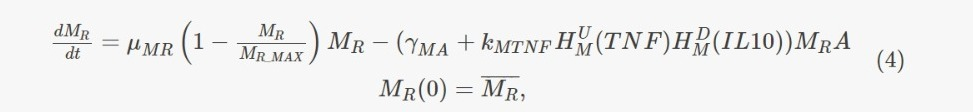
\includegraphics{images/397ab830-736c-47a6-881a-0279fd5025aa-01.jpg}

Estan los efectos de las citocinas que impactan a el parametro
\(K_{MTNF}\) que es: Activation rate of resting macrophages influenced
by TNF-α

El factor \(\gamma _{MA}\) es el factor de represents macrophage
activation at the rate γMA in response to the bacteria

TODO JUNTO: represents macrophage activation at the rate γMA in response
to the bacteria and activation rate kMTNF considering the influence of
the cytokines TNF and IL-10.

\hypertarget{segundo-modelo-con-citocinas}{%
\section{Segundo Modelo (Con
citocinas)}\label{segundo-modelo-con-citocinas}}

Se implementara la misma funcion de citocinas como en el modelo de
Staphylococcus aureus.

1.-\[ d{T_{L}} = \alpha_{1} T_{L} - (\alpha_{2} H_{M}^U(TNF)H_{M}^D(IL10)) T_{L}M_{\phi} - \alpha_{3}T_{L}C_{N} - \mu_{1} T_{L} \]

2.-\[ dT_{i} = (\alpha_{2} H_{M}^{U}(TNF)H_{M}^{D}(IL10)) T_{L}M_{\phi} + \alpha_{3}T_{L}C_{N} - (\alpha_{4}H_{M}^{U}(TNF)H_{M}^{U}(IFN)H_{M}^{D}(IL10) )M_{\phi}iT_{i}\]
\[-(\alpha_{5}H_{CD8}^{U}H_{CD8}^{D}(IL10))M_{\phi}iCD8 - (\alpha_{6}H_{CD8}^{U}(TNF)H_{CD8}^{U}(IFN)H_{CD8}^{D}(IL10))C_{i}CD8 - \mu_{2} T_{i} + \alpha_{9}T_{i} \]

3.-\[ dM_{\phi} = \alpha_{7}M_{\phi} - (\alpha_{2}H_{M}^{U}(TNF)H_{M}^{D}(IL10) )T_{L}M_{\phi} - \mu_{3} M_{\phi} \]

4-.\[ dM_{\phi}i = (\alpha_{2}H_{M}^{U}(TNF)H_{M}^{D}(IL10))T_{L}M_{\phi} - (\alpha_{5} H_{CD8}^{U}(IFN)H_{CD8}^{D}(IL10))M_{\phi}iCD8 -\mu_{4} M_{\phi}i \]

5.-\[ dC_{N}= \alpha_{8}C_{N} - \alpha_{3}T_{L}C_{N} - \mu_{5} C_{N} \]

6.-\[ dC_{i} = \alpha_{3}T_{L}C_{N} - (\alpha_{6} H_{CD8}^{U}(TNF)H_{CD8}^{U}(IFN)H_{CD8}^{D}(IL10))C_{i}CD8 - \mu_{6} C_{i} \]

7.-
\[ dCD8 = (\alpha_{10}H_{CD8}^{U}(IFN)H_{CD8}^{D}(IL10)) CD8 - (\mu_{7}H_{CD8}^{D}(IFN)H_{CD8}^{U}(IL10) )CD8 \]

8.-
\[dTNF = (\alpha_{11}H_{TNF}^{D}(IL10))M_{\phi}i - \mu_{8}(TNF - qTNF)\]

9.- \[ dIFN = (\alpha_{12}H_{IFN}^{D}(IL10))- \mu_{9}(IFN-qIFN)  \]

10.- \[dIL10 = \alpha_{13} - \mu_{10}(IL10-qIL10)  \]

\hypertarget{tercer-modelo-citocinas-y-retardos-de-priliferacion}{%
\section{Tercer Modelo (Citocinas y retardos de
priliferacion)}\label{tercer-modelo-citocinas-y-retardos-de-priliferacion}}

1.-\[ \dot{T_{L}} = (\alpha_{1} + \mu C_{i} + \mu M_{\phi}i) T_{L} - (\alpha_{2} H_{M}^U(TNF)H_{M}^D(IL10)) T_{L}M_{\phi} - \alpha_{3}T_{L}C_{N} - \mu_{1} T_{L} \]

2.-\[ \dot{T_{i}} = (\alpha_{2} H_{M}^{U}(TNF)H_{M}^{D}(IL10)) T_{L}M_{\phi} + \alpha_{3}T_{L}C_{N} - (\alpha_{4}H_{M}^{U}(TNF)H_{M}^{U}(IFN)H_{M}^{D}(IL10) )M_{\phi}iT_{i}\]
\[-(\alpha_{5}H_{CD8}^{U}H_{CD8}^{D}(IL10))M_{\phi}iCD8 - (\alpha_{6}H_{CD8}^{U}(TNF)H_{CD8}^{U}(IFN)H_{CD8}^{D}(IL10))C_{i}CD8 - \mu_{2} T_{i} + \alpha_{9}T_{i}(C_{i}+M_{\phi}i) \]

3.-\[ \dot {M_{\phi}} = \alpha_{7}(M_{\phi}-M_{\phi}0) - (\alpha_{2}H_{M}^{U}(TNF)H_{M}^{D}(IL10) )T_{L}M_{\phi} - \mu_{3} M_{\phi} \]

4-.\[ \dot{M_{\phi}i} = (\alpha_{2}H_{M}^{U}(TNF)H_{M}^{D}(IL10))T_{L}M_{\phi} - (\alpha_{5} H_{CD8}^{U}(IFN)H_{CD8}^{D}(IL10))M_{\phi}iCD8 -\mu_{4} M_{\phi}i \]

5.-\[ \dot{C_{N}}= \alpha_{8}(C_{N}-C_{N}0) - \alpha_{3}T_{L}C_{N} - \mu_{5} C_{N} \]

6.-\[ \dot{C_{i}} = \alpha_{3}T_{L}C_{N} - (\alpha_{6} H_{CD8}^{U}(TNF)H_{CD8}^{U}(IFN)H_{CD8}^{D}(IL10))C_{i}CD8 - \mu_{6} C_{i} \]

7.-
\[ \dot{CD8} = (\alpha_{10}H_{CD8}^{U}(IFN)H_{CD8}^{D}(IL10)) CD8 - (\mu_{7}H_{CD8}^{D}(IFN)H_{CD8}^{U}(IL10) )CD8 \]

8.-
\[\dot{TNF} = (\alpha_{11}H_{TNF}^{D}(IL10))M_{\phi}i - \mu_{8}(TNF - qTNF)\]

9.- \[ \dot{IFN} = (\alpha_{12}H_{IFN}^{D}(IL10))- \mu_{9}(IFN-qIFN)  \]

10.- \[\dot{IL10} = \alpha_{13} - \mu_{10}(IL10-qIL10)  \]

\begin{longtable}[]{@{}
  >{\raggedright\arraybackslash}p{(\columnwidth - 6\tabcolsep) * \real{0.2817}}
  >{\raggedright\arraybackslash}p{(\columnwidth - 6\tabcolsep) * \real{0.2394}}
  >{\raggedright\arraybackslash}p{(\columnwidth - 6\tabcolsep) * \real{0.2394}}
  >{\raggedright\arraybackslash}p{(\columnwidth - 6\tabcolsep) * \real{0.2394}}@{}}
\toprule\noalign{}
\begin{minipage}[b]{\linewidth}\raggedright
Variable
\end{minipage} & \begin{minipage}[b]{\linewidth}\raggedright
Valor Inicial
\end{minipage} & \begin{minipage}[b]{\linewidth}\raggedright
Definicion
\end{minipage} & \begin{minipage}[b]{\linewidth}\raggedright
Cita
\end{minipage} \\
\midrule\noalign{}
\endhead
\bottomrule\noalign{}
\endlastfoot
\(T_{L}\) & 50 & Parasitos en sangre & Freitas 2018 \\
\(T_{i}\) & 0 & Parasitos intracelulares & \\
\(M_{\phi}\) & 209 & Macrofagos & Freitas 2018 \\
\(M_{\phi i}\) & 0 & Macrofagos infectados & -------- \\
\(C_{N}\) & 136 & Cardiomiocitos no infectados & Freitas 2018 \\
\(C_{i}\) & 0 & Cardiomiocitos infectados & Freitas 2018 \\
CD8 & 708 & Linfocitos CD8 & Freitas 2018 \\
TNF & 0.14 & TNF alpha & Brady et al 2016 \\
IFN & 0.10 & IFN gamma & Rincon 2024 \\
IL10 & 0.15 & Interleucina 10 & Brady et al 2016 \\
\end{longtable}

\begin{longtable}[]{@{}
  >{\raggedright\arraybackslash}p{(\columnwidth - 6\tabcolsep) * \real{0.2703}}
  >{\raggedright\arraybackslash}p{(\columnwidth - 6\tabcolsep) * \real{0.2432}}
  >{\raggedright\arraybackslash}p{(\columnwidth - 6\tabcolsep) * \real{0.2432}}
  >{\raggedright\arraybackslash}p{(\columnwidth - 6\tabcolsep) * \real{0.2432}}@{}}
\toprule\noalign{}
\begin{minipage}[b]{\linewidth}\raggedright
Parametro
\end{minipage} & \begin{minipage}[b]{\linewidth}\raggedright
Valor
\end{minipage} & \begin{minipage}[b]{\linewidth}\raggedright
Definicion
\end{minipage} & \begin{minipage}[b]{\linewidth}\raggedright
Referencia
\end{minipage} \\
\midrule\noalign{}
\endhead
\bottomrule\noalign{}
\endlastfoot
\(\alpha_{1}\) & ---------------- & Tasa de entrada de parasitos &
-------------- \\
\(\alpha_{2}\) & ---------------- & Tasa de infeccion de macrofagos &
-------------- \\
\(\alpha_{3}\) & ---------------- & Tasa de infeccion de cardiomiocitos
& -------------- \\
\(\alpha_{4}\) & - & Tasa de eliminacion de parasito I por macrofago &
-------------- \\
\(\alpha_{5}\) & ---------------- & Tasa de eliminacion de Macrofago I
por CD8 & \\
\(\alpha_{6}\) & ---------------- & Tasa de eliminacion de cardiomiocito
I por CD8 & -- \\
\(\alpha_{7}\) & ---------------- & Tasa de produccion de Macrofagos &
-------------- \\
\(\alpha_{8}\) & ---------------- & Tasa de produccion de cardiomiocitos
& ---- \\
\(\alpha_{9}\) & ---------------- & Tasa de proliferacion del parasito I
& ----------- \\
\(\alpha_{10}\) & ---------------- & Tasa de proliferacion de CD8 &
-------------- \\
\(\alpha_{11}\) & ---------------- & Tasa de produccion de TNF &
-------------- \\
\(\alpha_{12}\) & ---------------- & Tasa de produccion de IFN &
-------------- \\
\(\alpha_{13}\) & ---------------- & Tasa de produccion IL-10 &
-------------- \\
\(\mu_{1}\) & ---------------- & Muerte de parasito libre &
-------------- \\
\(\mu_{2}\) & ---------------- & Muerte de Parasito intracelular &
-------------- \\
\(\mu_{3}\) & ---------------- & Muerte de macrofago & -------------- \\
\(\mu_{4}\) & ---------------- & Muerte de macrofago infectado &
-------------- \\
\(\mu_{5}\) & ---------------- & Muerte de cardiomiocito &
-------------- \\
\(\mu_{6}\) & ---------------- & Muerte de cardiomiocito infectado &
-------------- \\
\(\mu_{7}\) & ---------------- & Muerte de CD8 & -------------- \\
\(\mu_{8}\) & ---------------- & Caida de TNF & -------------- \\
\(\mu_{9}\) & ---------------- & Caida de IFN & -------------- \\
\(\mu_{10}\) & ---------------- & Caida de IL-10 & -------------- \\
\$ \$ & ---------------- & Caida de IL-10 & -------------- \\
\end{longtable}

Tienen parametros de produccion de citokinas por cada tipo celular o
estimulacion por otra citokina

\hypertarget{tercer-modelo-citocinas-y-funciones-de-hill}{%
\section{Tercer modelo Citocinas y funciones de
Hill}\label{tercer-modelo-citocinas-y-funciones-de-hill}}

1 .-
\[ \dot T_{L}= (\alpha_{1}+ \mu_{6} C_{i} + \mu_{4}M_{\phi i})T_{L} - [\alpha_{2}(\dfrac{TNF^{h}}{\eta^{h}(M)(TNF)+TNF^{h}}) (\dfrac{\eta^{h}(M)(IL10)}{\eta^{h}(M)(IL10)+IL10^{h}})]T_{L}M_{\phi} - \alpha_{3}T_{L}C_{N}-\mu_{1}T_{L}\]

2.-
\[\dot{T_{i}} = [\alpha_{2}(\dfrac{TNF^{h}}{\eta^{h}(M)(TNF)+TNF^{h}})(\dfrac{\eta^{h}(M)(IL10)}{\eta^{h}(M)(IL10)+IL10^{h}})]T_{L}M_{\phi}+ \alpha_{3}T_{L}C_{N} \]
\[- [\alpha_{4} (\dfrac{IFN^{h}}{\eta^{h}(M)(IFN)+IFN^{h}})(\dfrac{\eta^{h}(M)(IL10)}{\eta^{h}(M)(IL10)+IL10^{h}})(\dfrac{TNF^{h}}{\eta^{h}(M)(TNF)+TNF^{h}})]M_{\phi i}T_{i}\]
\[-[\alpha_{5}(\dfrac{IFN^{h}}{\eta^{h}(CD8)(IFN)+IFN^{h}})(\dfrac{\eta^{h}(CD8)(IL10)}{\eta^{h}(CD8)(IL10)+IL10^{h}})]M_{\phi i}CD8 \]
\[-[\alpha_{6}(\dfrac{TNF^{h}}{\eta^{h}(CD8)(TNF)+TNF^{h}})(\dfrac{IFN^{h}}{\eta^{h}(CD8)(IFN)+IFN^{h}})(\dfrac{\eta^{h}(CD8)(IL10)}{\eta^{h}(CD8)(IL10)+IL10^{h}})]C_{i}CD8 
\] \[- \mu_{2}T_{i}+ \alpha_{9}T_{i}(C_{i}+M_{\phi i}) \]
3.-\[ \dot{M_{\phi}}= \alpha_{7}(M_{\phi}-M_{\phi}0) - [\alpha_{2}(\dfrac{TNF^{h}}{\eta^{h}(M)(TNF)+TNF^{h}})(\dfrac{\eta^{h}(M)(IL10)}{\eta^{h}(M)(IL10)+IL10^{h}})]T_{L}M_{\phi}-\mu_{3}M_{\phi} \]

4.-
\[ \dot{M_{\phi i }}= [\alpha_{2}(\dfrac{TNF^{h}}{\eta^{h}(M)(TNF)+ TNF^{h}})(\dfrac{\eta^{h}(M)(IL10)}{\eta^{h}(M)(IL10)+IL10^{h}})]T_{L}M_{\phi} \]
\[-[\alpha_{5}(\dfrac{IFN^{h}}{\eta^{h}(CD8)(IFN)+IFN^{h}})(\dfrac{\eta^{h}(CD8)(IL10)}{\eta^{h}(CD8)(IL10)+IL10^{h}})]M_{\phi i }CD8 - \mu_{4}M_{\phi i} \]
5.-
\[\dot{C_{N}}= \alpha_{8}(C_{N}-C_{N}0) -\alpha_{3}T_{L}C_{N}-\mu_{5}C_{N} \]

6.-
\[ \dot{C_{i}}= \alpha_{3}T_{L}C_{N} - [\alpha_{6}(\dfrac{TNF^{h}}{\eta^{h}(CD8)(TNF)+TNF^{h}})(\dfrac{IFN^{h}}{\eta^{h}(CD8)(IFN)+IFN^{h}})(\dfrac{\eta^{h}(CD8)(IL10)}{\eta^{h}(CD8)(IL10)+ IL10^{h}})]C_{i}CD8 -\mu_{6}C_{i} \]

7.-
\[ \dot{ CD8}= [\alpha_{10}(\dfrac{IFN^{h}}{\eta^{h}(CD8)(IFN)+IFN^{h}})(\dfrac{\eta^{h}(CD8)(IL10)}{\eta^{h}(CD8)(IL10)+IL10^{h}})](CD8-CD80) \]
\[ -[\mu_{7}(\dfrac{IFN^{h}}{\eta^{h}(CD8)(IFN)+IFN^{h}})(\dfrac{\eta^{h}(CD8)(IL10)}{\eta^{h}(CD8)(IL10)+IL10^{h}})]\]
8.-
\[\dot{TNF}= [\alpha_{11}(\dfrac{\eta^{h}(TNF)(IL10)}{\eta^{h}(TNF)(IL10)+IL10^{h}})]M_{\phi i} - \mu_{8}(TNF-qTNF)  \]
9.-
\[\dot{IFN}= [\alpha_{12}(\dfrac{\eta^{h}(IFN)(IL10)}{\eta^{h}(IFN)(IL10)+ IL10^{h}})]C_{i}??? - \mu_{9}(IFN-qIFN) \]

10.-

\[\dot{IL10}= \alpha_{13}- \mu_{10}(IL10-qIL10) \]

\hypertarget{diagrama}{%
\section{Diagrama}\label{diagrama}}

\includegraphics{images/Modelo_citocinas.jfif}

\hypertarget{modelo-sin-cd8-desde-el-diagrama}{%
\section{Modelo sin CD8 desde el
diagrama}\label{modelo-sin-cd8-desde-el-diagrama}}

\begin{enumerate}
\def\labelenumi{\arabic{enumi}.}
\tightlist
\item
\end{enumerate}

\[ \dot{T_{L}}= \nu - [\alpha_{1}(\dfrac{TNF^{h}}{\eta^{h}(M)(TNF)+ TNF^{h}})(\dfrac{\eta^{h}(M)(IL10)}{\eta^{h}(M)(IL10)+IL10^{h}})]T_{L}M  \]
\[-\alpha_{2}T_{L}C_{N}- [\mu_{1}(\dfrac{TNF^{h}}{\eta^{h}(T_{L})(TNF)+TNF^{h}})(\dfrac{IFN^{h}}{\eta^{h}(T_{L})(IFN)+IFN^{h}})(\dfrac{\eta^{h}(T_{L})(IL10)}{\eta^{h}(T_{L})(IL10)+IL10^{h}})]T_{L} \]

\begin{enumerate}
\def\labelenumi{\arabic{enumi}.}
\setcounter{enumi}{1}
\tightlist
\item
\end{enumerate}

\[ \dot{M}= [\nu_{2}(\dfrac{TNF^{h}}{\eta^{h}(M)(TNF)+TNF^{h}})(\dfrac{\eta^{h}(M)(IL10)}{\eta^{h}(M)(IL10)+IL10^{h}})](M-M0)\]
\[-[\alpha_{1}(\dfrac{TNF^{h}}{\eta^{h}(M)(TNF)+ TNF^{h}})(\dfrac{\eta^{h}(M)(IL10)}{\eta^{h}(M)(IL10)+IL10^{h}})]T_{L}M\]
\[-[\mu_{2}(\dfrac{TNF^{h}}{\eta^{h}(M)(TNF)+TNF^{h}})(\dfrac{\eta^{h}(M)(IL10)}{\eta^{h}(M)(IL10)+IL10^{h}})]M  \]

\begin{enumerate}
\def\labelenumi{\arabic{enumi}.}
\setcounter{enumi}{2}
\tightlist
\item
\end{enumerate}

\[ \dot{C_{N}}= -\alpha_{2}T_{L}C_{N}-[\mu_{3}(\dfrac{TNF^{h}}{\eta^{h}(C_{N})(TNF)+TNF^{h}})(\dfrac{IFN^{h}}{\eta^{h}(C_{N})(IFN)+IL10^{h}})(\dfrac{\eta^{h}(C_{N})(IL10)}{\eta^{h}(C_{N})(IL10)+IL10^{h}})]C_{N} \]

\begin{enumerate}
\def\labelenumi{\arabic{enumi}.}
\setcounter{enumi}{3}
\tightlist
\item
\end{enumerate}

\[ \dot{T_{i}}=\alpha_{2}T_{L}C_{N}+[\alpha_{1}(\dfrac{TNF^{h}}{\eta^{h}(M)(TNF)+ TNF^{h}})(\dfrac{\eta^{h}(M)(IL10)}{\eta^{h}(M)(IL10)+IL10^{h}})]T_{L}M  \]
\[-[\mu_{4}(\dfrac{TNF^{h}}{\eta^{h}(M)(TNF)+TNF^{h}})(\dfrac{IFN^{h}}{\eta^{h}(M)(IFN)+IFN^{h}})(\dfrac{\eta^{h}(M)(IL10)}{\eta^{h}(M)(IL10)+IL10^{h}})]T_{i} \]
\[+[(\dfrac{TNF^{h}}{\eta^{h}(T_{i})(TNF)+TNF^{h}})(\dfrac{IFN^{h}}{\eta^{h}(T_{i})(IFN)+IFN^{h}})(\dfrac{\eta^{h}(T_{i})(IL10)}{\eta^{h}(T_{i})(IL10)+IL10^{h}})(\alpha_{3}+\alpha_{4})]T_{i}  \]

\begin{enumerate}
\def\labelenumi{\arabic{enumi}.}
\setcounter{enumi}{4}
\tightlist
\item
\end{enumerate}

\[ \dot{M_{i}}= +[\alpha_{1}(\dfrac{TNF^{h}}{\eta^{h}(T_{L})(TNF)+TNF^{h}})(\dfrac{\eta^{h}(T_{L})(IL10)}{\eta^{h}(T_{L})(IL10)+IL10^{h}})]T_{L}M   \]
\[-[\mu_{5}(\dfrac{IFN^{h}}{\eta^{h}(M)(IFN)+IFN^{h}})(\dfrac{\eta^{h}(M)(IL10)}{\eta^{h}(M)(IL10)+IL10^{h}}]M_{i}  \]

\begin{enumerate}
\def\labelenumi{\arabic{enumi}.}
\setcounter{enumi}{5}
\tightlist
\item
\end{enumerate}

\[ \dot{C_{i}}= +\alpha_{2}T_{L}C_{N}- [\mu_{6}(\dfrac{TNF^{h}}{\eta^{h}(C_{i})(TNF)+TNF^{h}})(\dfrac{IFN^{h}}{\eta^{h}(C_{i})(IFN)+IFN^{h}})(\dfrac{\eta^{h}(C_{I})(IL10)}{\eta^{h}(C_{i})(IL10)+IL10^{h}})]C_{i} \]

\begin{enumerate}
\def\labelenumi{\arabic{enumi}.}
\setcounter{enumi}{6}
\tightlist
\item
\end{enumerate}

\[\dot{TNF}= [\alpha_{5}(\dfrac{\eta^{h}(TNF)(IL10)}{\eta^{h}(TNF)(IL10)+IL10^{h}})]M_{i} -\mu_{7}(TNF -qTNF)\]

\begin{enumerate}
\def\labelenumi{\arabic{enumi}.}
\setcounter{enumi}{7}
\tightlist
\item
\end{enumerate}

\[ \dot{IFN}=  [\alpha_{6}(\dfrac{\eta^{h}(IFN)(IL10)}{\eta^{h}(IFN)(IL10)+IL10^{h}})]C_{i}-\mu_{8}(IFN-qIFN) \]

\begin{enumerate}
\def\labelenumi{\arabic{enumi}.}
\setcounter{enumi}{8}
\tightlist
\item
\end{enumerate}

\[ \dot{IL10}= \alpha{7}-\mu_{9}(IL10-qIL10) \]

\begin{longtable}[]{@{}
  >{\raggedright\arraybackslash}p{(\columnwidth - 6\tabcolsep) * \real{0.2817}}
  >{\raggedright\arraybackslash}p{(\columnwidth - 6\tabcolsep) * \real{0.2394}}
  >{\raggedright\arraybackslash}p{(\columnwidth - 6\tabcolsep) * \real{0.2394}}
  >{\raggedright\arraybackslash}p{(\columnwidth - 6\tabcolsep) * \real{0.2394}}@{}}
\toprule\noalign{}
\begin{minipage}[b]{\linewidth}\raggedright
Variable
\end{minipage} & \begin{minipage}[b]{\linewidth}\raggedright
Valor Inicial
\end{minipage} & \begin{minipage}[b]{\linewidth}\raggedright
Definicion
\end{minipage} & \begin{minipage}[b]{\linewidth}\raggedright
Cita
\end{minipage} \\
\midrule\noalign{}
\endhead
\bottomrule\noalign{}
\endlastfoot
\(T_{L}\) & 50 & Parasitos en sangre & Freitas 2018 \\
\(T_{i}\) & 0 & Parasitos intracelulares & --------------- \\
\(M_{\phi}\) & 209 & Macrofagos & Freitas 2018 \\
\(M_{\phi i}\) & 0 & Macrofagos infectados & -------- \\
\(C_{N}\) & 136 & Cardiomiocitos no infectados & Freitas 2018 \\
\(C_{i}\) & 0 & Cardiomiocitos infectados & Freitas 2018 \\
TNF & 0.14 & TNF alpha & Brady et al 2016 \\
IFN & 0.10 & IFN gamma & Rincon 2024 \\
IL10 & 0.15 & Interleucina 10 & Brady et al 2016 \\
\end{longtable}

\begin{longtable}[]{@{}
  >{\raggedright\arraybackslash}p{(\columnwidth - 6\tabcolsep) * \real{0.2703}}
  >{\raggedright\arraybackslash}p{(\columnwidth - 6\tabcolsep) * \real{0.2432}}
  >{\raggedright\arraybackslash}p{(\columnwidth - 6\tabcolsep) * \real{0.2432}}
  >{\raggedright\arraybackslash}p{(\columnwidth - 6\tabcolsep) * \real{0.2432}}@{}}
\toprule\noalign{}
\begin{minipage}[b]{\linewidth}\raggedright
Parametro
\end{minipage} & \begin{minipage}[b]{\linewidth}\raggedright
Valor
\end{minipage} & \begin{minipage}[b]{\linewidth}\raggedright
Definicion
\end{minipage} & \begin{minipage}[b]{\linewidth}\raggedright
Referencia
\end{minipage} \\
\midrule\noalign{}
\endhead
\bottomrule\noalign{}
\endlastfoot
\(\alpha_{1}\) & \(3.14X^{-10} \dfrac{1}{M_{\phi}*Dia}\) & Tasa de
fagocitosis de Macrofagos & Flores Garza 2022 \\
\(\alpha_{2}\) & \(2.5X10^{-9}\) & Tasa de infeccion de cardiomiocitos &
Freitas 2018 \\
\(\mu_{1}\)* & \(0.06 \dfrac{1}{Dia}\) & Muerte de pareasito libre &
Yang 2015 \\
\(\mu_{1}\)* & \(1X10^{-1}\) & Muerte de pareasito libre & Freitas
2018 \\
\(\nu_{2}\)* & 1 & Proliferacion de Macrofagos & Freitas 2018 \\
\(\nu_{2}\)* & 1,080,728 & Proliferacion de Macrofagos & Flores Garza
2022 \\
\(\mu_{2}\) & \(0.0019 \dfrac{1}{Dia}\) & Tasa de muerte de macrofago &
Flores Garza 2022 \\
\(\mu_{2}\) & \(5X10^{-1}\) & Tasa de muerte de macrofago & Freitas
2018 \\
\(\mu_{3}\) & ----------------- & Muerte de cardiomiocitos &
----------------- \\
\(\mu_{4}\) & \(5X10^{-4} + 1.5X10^{-4}\) & Tasa de muerte de
Trypanosoma intracelular & Freitas 2018 (M+CD8) \\
\(\alpha_{3}\)* & 90 & Tasa de proliferacion en \(C_{i}\) & Freitas
2018 \\
\(\alpha_{3}\)* & \(20 \dfrac{1}{Ti*Sc}\) & Tasa de proliferacion en
\(C_{i}\) & Yang 2015 Sc=Susceptible cells \\
\(\alpha_{3}\)* & 1.95 * cell & Tasa de proliferacion en \(C_{i}\) &
Arias 2020 \\
\(\alpha_{4}\)* & 90 & Tasa de proliferacion en \(M_{i}\) & Freitas
2018 \\
\(\alpha_{4}\)* & \(20 \dfrac{1}{Ti*Sc}\) & Tasa de proliferacion en
\(M_{i}\) & Yang 2015 Sc=Susceptible cells \\
\(\alpha_{4}\)* & 1.95 * cell & Tasa de proliferacion en \(M_{i}\) &
Arias 2020 \\
\(\mu_{5}\) & \(5X10^{-1}\) & Muerte de Macrofago infectado & Feitas
2018 \\
\(\mu_{6}\) & \(1X10^{-6}\) & Muerte de cardiomiocito infectado &
Freitas 2018 \\
\(\alpha_{5}\) & \(200 \dfrac{1}{Dia} + 1.5 \dfrac{1}{M*Dia}\) &
Secrecion de TNF-\(\alpha\) & Talaei 2021 \\
\(\alpha_{6}\) & ----------------- & Secrecion de IFN-\(\gamma\) &
----------------- \\
\(\alpha_{7}\) & \(1.1 \dfrac{1}{Dia} + 0.19 \dfrac{R}{Dia*M}\) &
Secrecion de IL-10 & Talaei 2021 \\
\(\mu_{7}\) & ----------------- & Degradacion de TNF-\(\alpha\) &
----------------- \\
\(\mu_{8}\) & ----------------- & Degradacion de IFN-\(\gamma\) &
----------------- \\
\(\mu_{9}\) & ----------------- & Degradacion de IL-10 &
----------------- \\
\(\eta_{TNF-IL10}\) & 17.4 & Hill Functions Relative concentration &
Talaei 2021 \\
\(\eta_{10-IL6}\) & 560 & Hill Functions Relative concentration & Talaei
2021 \\
\(h_{10-IL6}\) & 3.68 & Hill Functions Dimentionless & Talaei 2021 \\
\(h_{TNF-IL10}\) & 3 & Hill Functions Dimentionless & Talaei 2021 \\
\end{longtable}

\hypertarget{modelo-corregido}{%
\section{Modelo corregido}\label{modelo-corregido}}

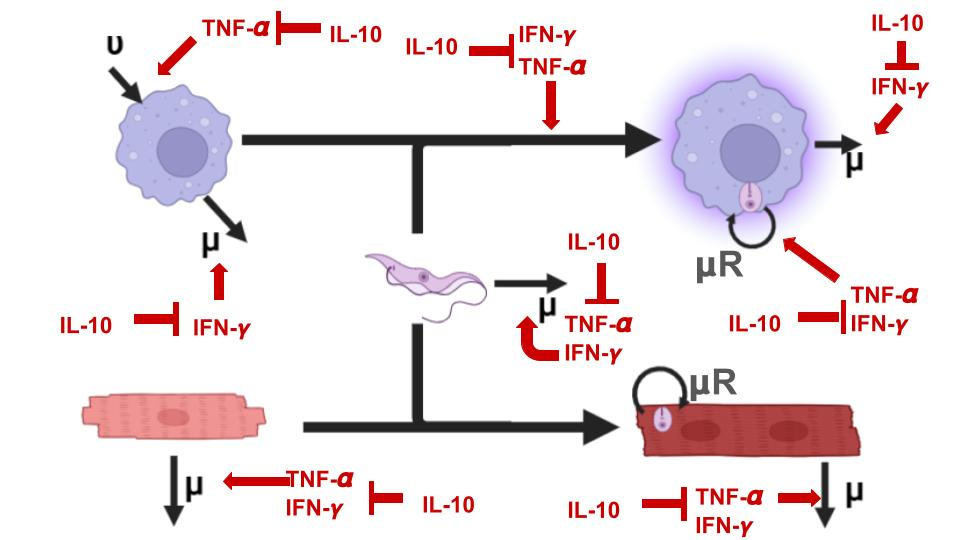
\includegraphics{images/Proyecto de Tesis.jpg}

\hypertarget{poster-oaxaca}{%
\section{POSTER OAXACA}\label{poster-oaxaca}}

\hypertarget{ecuaciones-de-modelo-corregido}{%
\subsection{Ecuaciones de Modelo
corregido}\label{ecuaciones-de-modelo-corregido}}

\begin{enumerate}
\def\labelenumi{\arabic{enumi}.}
\tightlist
\item
\end{enumerate}

\[ \dot{T_{L}}= - [\alpha_{1}(\dfrac{TNF^{h}}{\eta^{h}(M)(TNF)+ TNF^{h}})(\dfrac{IFN^{h}}{\eta^{h}(M)(IFN)+IFN^{h}})(\dfrac{\eta^{h}(M)(IL10)}{\eta^{h}(M)(IL10)+IL10^{h}})]T_{L}M  \]
\[-\alpha_{2}T_{L}C_{N}- [\mu_{1}(\dfrac{TNF^{h}}{\eta^{h}(T_{L})(TNF)+TNF^{h}})(\dfrac{IFN^{h}}{\eta^{h}(T_{L})(IFN)+IFN^{h}})(\dfrac{\eta^{h}(T_{L})(IL10)}{\eta^{h}(T_{L})(IL10)+IL10^{h}})]T_{L} \]

\begin{enumerate}
\def\labelenumi{\arabic{enumi}.}
\setcounter{enumi}{1}
\tightlist
\item
\end{enumerate}

\[ \dot{M}= [\nu_{2}(\dfrac{TNF^{h}}{\eta^{h}(M)(TNF)+TNF^{h}})(\dfrac{\eta^{h}(M)(IL10)}{\eta^{h}(M)(IL10)+IL10^{h}})](M-M0)\]
\[-[\alpha_{1}(\dfrac{TNF^{h}}{\eta^{h}(M)(TNF)+ TNF^{h}})(\dfrac{IFN^{h}}{\eta^{h}(M)(IFN)+IFN^{h}})(\dfrac{\eta^{h}(M)(IL10)}{\eta^{h}(M)(IL10)+IL10^{h}})]T_{L}M\]
\[-[\mu_{2}(\dfrac{IFN^{h}}{\eta^{h}(M)(IFN)+IFN^{h}})(\dfrac{\eta^{h}(M)(IL10)}{\eta^{h}(M)(IL10)+IL10^{h}})]M  \]

\begin{enumerate}
\def\labelenumi{\arabic{enumi}.}
\setcounter{enumi}{2}
\tightlist
\item
\end{enumerate}

\[ \dot{C_{N}}= -\alpha_{2}T_{L}C_{N}-[\mu_{3}(\dfrac{IFN^{h}}{\eta^{h}(C_{N})(IFN)+IFN^{h}})(\dfrac{\eta^{h}(C_{N})(IL10)}{\eta^{h}(C_{N})(IL10)+IL10^{h}})]C_{N} \]

\begin{enumerate}
\def\labelenumi{\arabic{enumi}.}
\setcounter{enumi}{3}
\tightlist
\item
\end{enumerate}

\[ \dot{T_{i}}=\alpha_{2}T_{L}C_{N}+[\alpha_{1}(\dfrac{TNF^{h}}{\eta^{h}(M)(TNF)+ TNF^{h}})(\dfrac{IFN^{h}}{\eta^{h}(M)(IFN)+IFN^{h}})(\dfrac{\eta^{h}(M)(IL10)}{\eta^{h}(M)(IL10)+IL10^{h}})]T_{L}M  \]
\[-[\mu_{4}(\dfrac{TNF^{h}}{\eta^{h}(M)(TNF)+TNF^{h}})(\dfrac{IFN^{h}}{\eta^{h}(M)(IFN)+IFN^{h}})(\dfrac{\eta^{h}(M)(IL10)}{\eta^{h}(M)(IL10)+IL10^{h}})]T_{i} \]
\[+[(\dfrac{TNF^{h}}{\eta^{h}(T_{i})(TNF)+TNF^{h}})(\dfrac{IFN^{h}}{\eta^{h}(T_{i})(IFN)+IFN^{h}})(\dfrac{\eta^{h}(T_{i})(IL10)}{\eta^{h}(T_{i})(IL10)+IL10^{h}})(\alpha_{3}+\alpha_{4})]T_{i}  \]

\begin{enumerate}
\def\labelenumi{\arabic{enumi}.}
\setcounter{enumi}{4}
\tightlist
\item
\end{enumerate}

\[ \dot{M_{i}}= +[\alpha_{1}(\dfrac{TNF^{h}}{\eta^{h}(T_{L})(TNF)+TNF^{h}})(\dfrac{IFN^{h}}{\eta^{h}(M)(IFN)+IFN^{h}})(\dfrac{\eta^{h}(T_{L})(IL10)}{\eta^{h}(T_{L})(IL10)+IL10^{h}})]T_{L}M   \]
\[-[\mu_{5}(\dfrac{IFN^{h}}{\eta^{h}(M)(IFN)+IFN^{h}})(\dfrac{\eta^{h}(M)(IL10)}{\eta^{h}(M)(IL10)+IL10^{h}}]M_{i}  \]

\begin{enumerate}
\def\labelenumi{\arabic{enumi}.}
\setcounter{enumi}{5}
\tightlist
\item
\end{enumerate}

\[ \dot{C_{i}}= +\alpha_{2}T_{L}C_{N}- [\mu_{6}(\dfrac{TNF^{h}}{\eta^{h}(C_{i})(TNF)+TNF^{h}})(\dfrac{IFN^{h}}{\eta^{h}(C_{i})(IFN)+IFN^{h}})(\dfrac{\eta^{h}(C_{I})(IL10)}{\eta^{h}(C_{i})(IL10)+IL10^{h}})]C_{i} \]

\begin{enumerate}
\def\labelenumi{\arabic{enumi}.}
\setcounter{enumi}{6}
\tightlist
\item
\end{enumerate}

\[\dot{TNF}= [\alpha_{5}(\dfrac{\eta^{h}(TNF)(IL10)}{\eta^{h}(TNF)(IL10)+IL10^{h}})]M_{i} -\mu_{7}(TNF -qTNF)\]

\begin{enumerate}
\def\labelenumi{\arabic{enumi}.}
\setcounter{enumi}{7}
\tightlist
\item
\end{enumerate}

\[ \dot{IFN}=  [\alpha_{6}(\dfrac{\eta^{h}(IFN)(IL10)}{\eta^{h}(IFN)(IL10)+IL10^{h}})]C_{i}-\mu_{8}(IFN-qIFN) \]

\begin{enumerate}
\def\labelenumi{\arabic{enumi}.}
\setcounter{enumi}{8}
\tightlist
\item
\end{enumerate}

\[ \dot{IL10}= \alpha{7}-\mu_{9}(IL10-qIL10) \]

\hypertarget{explicacion-de-las-ecuaciones}{%
\section{Explicacion de las
ecuaciones}\label{explicacion-de-las-ecuaciones}}

\hypertarget{primer-ecuacion-tl.-trypanosomas-libres-poner-la-contribucion-de-los-que-salen-de-las-celulas}{%
\subsection{Primer ecuacion Tl. Trypanosomas Libres (PONER LA
CONTRIBUCION DE LOS QUE SALEN DE LAS
CELULAS)}\label{primer-ecuacion-tl.-trypanosomas-libres-poner-la-contribucion-de-los-que-salen-de-las-celulas}}

\[ - [\alpha_{1}(\dfrac{TNF^{h}}{\eta^{h}(M)(TNF)+ TNF^{h}})(\dfrac{\eta^{h}(M)(IL10)}{\eta^{h}(M)(IL10)+IL10^{h}})]T_{L}M  \]
Los trypomastigotes que se encutran en via sanguinea, van a interactuar
con los macrofagos (M) a una tasa \(\alpha_{1}\), por medio de la
fagocitosis, dejan de ser trypomanosomas libres y se vuelven
trypanosomas intracelulares. La fagocitosis de estos se ve impactado por
el ambiente de citocinas. En un ambiente proinflamatorio habra mas
fagocitosis que en un ambiente antiinflamatorio.

\[-\alpha_{2}T_{L}C_{N}\] Los trypanosomas libres invaden los
cardiomiocitos a una tasa \(\alpha_{2}\). Dejan de ser trypanosomas
libres y se vuelven trypanosomas intracelulares.

\[- [\mu_{1}(\dfrac{TNF^{h}}{\eta^{h}(T_{L})(TNF)+TNF^{h}})(\dfrac{IFN^{h}}{\eta^{h}(T_{L})(IFN)+IFN^{h}})(\dfrac{\eta^{h}(T_{L})(IL10)}{\eta^{h}(T_{L})(IL10)+IL10^{h}})]T_{L}\]
Los trypanosomas libres que se encuentran en via sanguinea, mueren a una
tasa \(\mu_{1}\), sin embargo se encuentran expuestos a otros
componentes del sistema inmune (neutrofilos, complemento, anticuerpos,
etc.) los cuales pueden incrementar su actvidad en un ambiente
proinflamatorio (\(TNF-\alpha \ y \ IFN-\gamma\)) que en un ambiente
antiinflamatorio (\(IL-10\)) aumentando latasa de muerte de trypanosomas
libres.

\hypertarget{segunda-ecuacion-m.-macrofagos-no-infectadossin-fagocitar}{%
\subsection{Segunda ecuacion M. Macrofagos no infectados/sin
fagocitar}\label{segunda-ecuacion-m.-macrofagos-no-infectadossin-fagocitar}}

\[ [\nu_{1}(\dfrac{TNF^{h}}{\eta^{h}(M)(TNF)+TNF^{h}})(\dfrac{\eta^{h}(M)(IL10)}{\eta^{h}(M)(IL10)+IL10^{h}})](M-M0)\]
Los macrofagos proliferan a una tasa \(\nu_{1}\), esta proliferacion
pueden aumentar dependiendo de su reclutamiento en un ambiente
proinflamatorio que en un ambiente antiinflamatorio. \((M-M0)\)
representa el retardo de proliferacion de los macrofagos.
\[-[\alpha_{1}(\dfrac{TNF^{h}}{\eta^{h}(M)(TNF)+ TNF^{h}})(\dfrac{\eta^{h}(M)(IL10)}{\eta^{h}(M)(IL10)+IL10^{h}})]T_{L}M\]
Los macrofagos sin infectar, interactuan con los trypanosomas libre, que
los fagocitan a una tasa \(\alpha_{1}\), esta tasa de fagocitosis
aumenta en presencia de citocinas proinflamatorias (\(TNF-\alpha\)) que
en presencia de citocinas antiinflamatorias \(IL-10\).

\[-[\mu_{2}(\dfrac{IFN^{h}}{\eta^{h}(M)(IFN)+IFN^{h}})(\dfrac{\eta^{h}(M)(IL10)}{\eta^{h}(M)(IL10)+IL10^{h}})]M\]
Los macrofagos no infectados o que no han fagocitado, mueren a una tasa
\(\mu_{2}\), esta muerte del macrofago se puede aumentar en presencia de
estres proinflamatorio como la citocina \(IFN-\gamma\) y verse el
efectuo reducida de esta con la citocina antiinflamatoria \(IL-10\)

\hypertarget{tercera-ecuacion-cn.-cardiomiocitos-no-infectados}{%
\subsection{Tercera ecuacion Cn. Cardiomiocitos no
infectados}\label{tercera-ecuacion-cn.-cardiomiocitos-no-infectados}}

\[-\alpha_{2}T_{L}C_{N}\] Los cardiomiocitos no infectados se infectan
por el trypanosoma a una tasa \(\alpha_{2}\), dejando de ser
cardiomiocitos no infectados y volviendose cardiomiocitos infectados

\[-[\mu_{3}(\dfrac{IFN^{h}}{\eta^{h}(C_{N})(IFN)+IL10^{h}})(\dfrac{\eta^{h}(C_{N})(IL10)}{\eta^{h}(C_{N})(IL10)+IL10^{h}})]C_{N} \]
Los cardiomiocitos no infectados mueren a una tasa \(\mu_{3}\), pero su
mortalidad puede aumentar en presencia de ambiente proinflamatorio
(\(INF-\gamma\)) o verse disminuida por un ambiente antiinflamatorio
(\(IFN-\gamma\))

\hypertarget{cuarta-ecuacion-ti.-trypanosoma-intracelular.}{%
\subsection{Cuarta ecuacion Ti. Trypanosoma
intracelular.}\label{cuarta-ecuacion-ti.-trypanosoma-intracelular.}}

\[\alpha_{2}T_{L}C_{N}\]

\[+[\alpha_{1}(\dfrac{TNF^{h}}{\eta^{h}(M)(TNF)+ TNF^{h}})(\dfrac{\eta^{h}(M)(IL10)}{\eta^{h}(M)(IL10)+IL10^{h}})]T_{L}M  \]
Lo trypanosomas libres que son fagocitados a una tasa \(\alpha_{1}\), se
convierten en trypanosomas intracelulares. La fagocitosis esta mediada
por el ambiente de citocinas proinflamatorias o antiinflamatorias

\[-[\mu_{4}(\dfrac{TNF^{h}}{\eta^{h}(M)(TNF)+TNF^{h}})(\dfrac{IFN^{h}}{\eta^{h}(M)(IFN)+IFN^{h}})(\dfrac{\eta^{h}(M)(IL10)}{\eta^{h}(M)(IL10)+IL10^{h}})]T_{i} \]
Los trypanosomas intracelulares, mueren a una tasa \(\mu_{4}\), esta
muerte de los parasitos intracelulares se puede ver afectada por el
sistema inmune, ya sea por su estimulacion a apoptosis, activacion de
linfocitos citotoxicos, mayor produccion de especies reactivas de
nitrogeno del macrofago, etc.

\[+[(\dfrac{TNF^{h}}{\eta^{h}(T_{i})(TNF)+TNF^{h}})(\dfrac{IFN^{h}}{\eta^{h}(T_{i})(IFN)+IFN^{h}})(\dfrac{\eta^{h}(T_{i})(IL10)}{\eta^{h}(T_{i})(IL10)+IL10^{h}})(\alpha_{3}+\alpha_{4})]T_{i}\]
Los trypomastigotes intracelulares se replican dentro la celula
hospedero, a una tasa de \(\alpha_{3}\) para los macrofagos y a una tasa
de \(\alpha_{4}\) en los cardiomiocitos, esta rpelicacion se puede ver
afectada por el ambiente de citocinas que pueden estimular produccion de
especies reactivas de nitrogeno, impidiendo la replicacion del parasito.
O con IL-10 que inhibe esta actividad antiparasitica. (VER EFECTO DE
CITOCINAS EN LA REPLICACION O SOLO EN SU MUERTE?)

\hypertarget{quinta-ecuacion-mi.-macrofago-infectado.}{%
\subsection{Quinta ecuacion Mi. Macrofago
infectado.}\label{quinta-ecuacion-mi.-macrofago-infectado.}}

\[+[\alpha_{1}(\dfrac{TNF^{h}}{\eta^{h}(T_{L})(TNF)+TNF^{h}})(\dfrac{\eta^{h}(T_{L})(IL10)}{\eta^{h}(T_{L})(IL10)+IL10^{h}})]T_{L}M   \]
Los macrofagos al interaccionar con el parasito y fagocitarlo a una tasa
\(\alpha_{1}\) se convierten en macrofagos infectados. Esta fagocitosis
se puede ver aumentada con citocinas proinflamatorias o disminuida con
citocinas antiinflamatorias

\[-[\mu_{5}(\dfrac{IFN^{h}}{\eta^{h}(M)(IFN)+IFN^{h}})(\dfrac{\eta^{h}(M)(IL10)}{\eta^{h}(M)(IL10)+IL10^{h}}]M_{i}  \]
Los macrofagos infectados, mueren a una tasa \(\mu_{5}\), esta tasa se
puede ver afectada por el ambiente inflamatorio, aumenta en presencia de
citocinas proinflamatorias que aumentan la apoptosis de las celulas
infectadas, o por citocinas antiinflamatorias que disminuyen la
apoptosis.

\hypertarget{sexta-ecuacion-ci.-cardiomiocito-infectado.}{%
\subsection{Sexta ecuacion Ci. Cardiomiocito
infectado.}\label{sexta-ecuacion-ci.-cardiomiocito-infectado.}}

\[+\alpha_{2}T_{L}C_{N}\] Los trypanosomas libres infectan a los
cardiomiocitos a una tasa \(\alpha_{2}\), de forma que se aumenta la
poblacion de cardiomiocitos infectados.

\[-[\mu_{6}(\dfrac{TNF^{h}}{\eta^{h}(C_{i})(TNF)+TNF^{h}})(\dfrac{IFN^{h}}{\eta^{h}(C_{i})(IFN)+IFN^{h}})(\dfrac{\eta^{h}(C_{I})(IL10)}{\eta^{h}(C_{i})(IL10)+IL10^{h}})]C_{i}\]
Los cardiomiocitos infectados mueren a una tasa \(\mu_{6}\), la cul se
puede ver aumentado por ambiente proinflamatorio y promover la
apoptosis, o inhibirlo con la presencia de citocinas antiiflamatorias

\hypertarget{septima-ecuacion-tnf.-factor-de-necrosis-tumoral-alpha-proinflamatoria}{%
\subsection{Septima ecuacion TNF. Factor de Necrosis Tumoral Alpha
(Proinflamatoria)}\label{septima-ecuacion-tnf.-factor-de-necrosis-tumoral-alpha-proinflamatoria}}

\[[\alpha_{5}(\dfrac{\eta^{h}(TNF)(IL10)}{\eta^{h}(TNF)(IL10)+IL10^{h}})]M_{i}\]
La citocina \(TNF-\alpha\) se secreta por los macrofagos a una tasa
\(\alpha_{5}\), aumentando su concentracion, esta secrecion de citocina
puede verse inhibida por la citocina antiinflamatoria IL-10

\[-\mu_{7}(TNF -qTNF)\] La citocina \(TNF-\alpha\) se degrada a una tasa
\(\mu_{7}\), pero no puede llegar a cero y unicamente puede llegar a su
nivel basal qTNF

\hypertarget{octava-ecuacion-ifn.-interferon-gamma}{%
\subsection{Octava ecuacion IFN. interferon
gamma}\label{octava-ecuacion-ifn.-interferon-gamma}}

\[[\alpha_{6}(\dfrac{\eta^{h}(IFN)(IL10)}{\eta^{h}(IFN)(IL10)+IL10^{h}})]C_{i}\]
La citocina \(IFN-\gamma\) es secretada a una tasa \(\mu_{6}\) por los
cardiomiocitos infectados, asi como otros grupos celulares, esta
produccion de interferon s epuede ver inhibida en la presencia de la
citocina antiinflamatoria IL-10.

\[-\mu_{8}(IFN-qIFN)\] La citocina se degrada a una tasa \(\mu_{8}\),
pero no puede llegar a cero, unicamente a su nivel basal qIFN

\hypertarget{novena-ecuacion-il10.-interleucina-10}{%
\subsection{Novena ecuacion IL10. Interleucina
10}\label{novena-ecuacion-il10.-interleucina-10}}

\[ \alpha{7}-\mu_{9}(IL10-qIL10) \] La citocina IL-10 se secreta a una
tasa \(\alpha_{7}\) y se degrada a una tasa \(\mu_{9}\), pero no puede
llegar a cero, unicamente a su nivel basal qIL10

\hypertarget{determinar-cuales-valores-de-las-citocinas-son-multiplicativos-y-cuales-son-agregativos-o-ambos}{%
\subsection{Determinar cuales valores de las citocinas son
multiplicativos y cuales son agregativos o
ambos}\label{determinar-cuales-valores-de-las-citocinas-son-multiplicativos-y-cuales-son-agregativos-o-ambos}}

\hypertarget{ecuacion-1}{%
\subsubsection{Ecuacion 1}\label{ecuacion-1}}

\(\alpha_{1}\) Es una interaccion multiplicativa, debido a que se tiene
una tasa de fagocitosis por parte del macrofago, la activacion de los
macrofagos por parte del ambiente pro-inflamatorio incrementa esta tasa
de fagocitosis, de una forma multiplicativa

\(\mu_{1}\) el efecto de las citocinas seria un efecto agregativo, de
igual forma puede ser un efecto multiplicativo si aumenta la tasa de
muerte por el estres al parasito. Sin embargo la mayor parte de muerte
de citocinas, se deberia a la activacion de componenetes celulares no
contemplados en el modelo, como pueden ser opsinizacion de anticuerpos,
opsonizacion del fragmento C3b del complemento, mayor proliferacion de
neutrofilos que ataquen al parasito, NETosis por parte de los
neutrofilos, mayor formacion de complejos de ataque a membrana (MAC) por
parte del complemento, etc. Estos factores incrementan la tasa de
fagocitosis sin afectar directamente en el mecanismo de muerte del
parasito.

\hypertarget{ecuacion-2}{%
\subsubsection{Ecuacion 2}\label{ecuacion-2}}

\(\nu_{1}\) hace una interaccion multiplicativa con las citocinas,
debido a que el ambiente pro-inflamatorio estimula la tasa de produccion
de macrofagos derivados de la medula osea, asi como facilitar su
migracion al sitio de infeccion con el parasito

\(\alpha_{1}\) se describio su interaccion en la ecuacion 1

\(\mu_{2}\) hace una interaccion multiplicativa con el ambiente de
citocinas,un incremento de citocina pro-inflamatoria como \(IFN-\gamma\)
aumenta la tasa de muerte del macrofago por medio de la estimulacion del
mecanismo de apoptosis.

\hypertarget{ecuacion-3}{%
\subsubsection{Ecuacion 3}\label{ecuacion-3}}

\(\mu_{3}\) hace una interaccion multiplicativo con las citocinas
implicadas, ya que debido al estres de las citocinas proinflamatorias,
los procesos de apoptosis aumentan.

\hypertarget{ecuacion-4}{%
\subsubsection{Ecuacion 4}\label{ecuacion-4}}

\(\alpha_{1}\) Se describio previamente en la ecuacion 1

\(\mu_{4}\) La muerte de los parasitos intracelulares, se afecta por las
citocinas de manera multiplicativa y aditivo. Multiplicativa, por que se
incrmentan la produccion de Oxido Nitrico en el caso de los Macrofagos
que aumentan la tasa de muerte (Aditivo?). Por otro lado un efecto
aditivo, debido a que los parasitos intracelulares mueren por la
activacion de las CD8, que eliminan a las celulas infectadas, como en el
caso de cardiomiocitos y macrofagos infectados

\(\alpha_{3} \ y \ \alpha_{4}\) Hace una interaccion con las citocinas
de manera multiplicativa, ya que la interaccion disminuye la replicacion
del parasito por estres

\hypertarget{quinta-ecuacion}{%
\subsubsection{Quinta ecuacion}\label{quinta-ecuacion}}

\(\alpha_{1}\) Se describio en la ecuacion 1

\(\alpha_{5}\) Las citocinas tendrian un efecto aditivo y
multiplicativo, pues un ambiente inflamatorio,de modo multiplicativo
aumenta la tasa de apoptosis por el estres celular y aditivo debido a
que activa los linfocitos CD8, que eliminan a las celulas infectadas

\hypertarget{ecuacion-6}{%
\subsubsection{Ecuacion 6}\label{ecuacion-6}}

\(\mu_{6}\) La muerte de los cardiomiocitos infectados su interaccion
con las citocinas es multiplicativo y aditivo. El efecto multiplicativo
por que elestres de las citocinas incrementa la tasa de apoptosis.
Efecto aditivo por la activacion de CD8 y destruccion de los
cardiomiocitos infectados

\hypertarget{para-tesis}{%
\section{PARA TESIS}\label{para-tesis}}

\hypertarget{ecuaciones-de-modelo-corregido-con-factores-aditivos-y-multiplicativos}{%
\subsection{Ecuaciones de Modelo corregido con factores aditivos y
multiplicativos}\label{ecuaciones-de-modelo-corregido-con-factores-aditivos-y-multiplicativos}}

\begin{enumerate}
\def\labelenumi{\arabic{enumi}.}
\tightlist
\item
\end{enumerate}

\[ \dot{T_{L}}= - [\alpha_{1}(\dfrac{TNF^{h}}{\eta^{h}(M)(TNF)+ TNF^{h}})(\dfrac{IFN^{h}}{\eta^{h}(M)(IFN)+IFN^{h}})(\dfrac{\eta^{h}(M)(IL10)}{\eta^{h}(M)(IL10)+IL10^{h}})]T_{L}M \]

\[-\alpha_{2}T_{L}C_{N}- [(\mu_{1}+1)((\dfrac{TNF^{h}}{\eta^{h}(T_{L})(TNF)+TNF^{h}})(\dfrac{IFN^{h}}{\eta^{h}(T_{L})(IFN)+IFN^{h}})(\dfrac{\eta^{h}(T_{L})(IL10)}{\eta^{h}(T_{L})(IL10)+IL10^{h}}))]T_{L} \]
\[+[(\mu_{5}+1)((\dfrac{IFN^{h}}{\eta^{h}(M)(IFN)+IFN^{h}})(\dfrac{\eta^{h}(M)(IL10)}{\eta^{h}(M)(IL10)+IL10^{h}}))]M_{i}\]
\[+[(\mu_{6}+1)((\dfrac{TNF^{h}}{\eta^{h}(C_{i})(TNF)+TNF^{h}})(\dfrac{IFN^{h}}{\eta^{h}(C_{i})(IFN)+IFN^{h}})(\dfrac{\eta^{h}(C_{I})(IL10)}{\eta^{h}(C_{i})(IL10)+IL10^{h}}))]C_{i} \]

\begin{enumerate}
\def\labelenumi{\arabic{enumi}.}
\setcounter{enumi}{1}
\tightlist
\item
\end{enumerate}

\[ \dot{M}= [\nu_{2}(\dfrac{TNF^{h}}{\eta^{h}(M)(TNF)+TNF^{h}})(\dfrac{\eta^{h}(M)(IL10)}{\eta^{h}(M)(IL10)+IL10^{h}})](M-M0)\]
\[-[\alpha_{1}(\dfrac{TNF^{h}}{\eta^{h}(M)(TNF)+ TNF^{h}})(\dfrac{IFN^{h}}{\eta^{h}(M)(IFN)+IFN^{h}})(\dfrac{\eta^{h}(M)(IL10)}{\eta^{h}(M)(IL10)+IL10^{h}})]T_{L}M\]
\[-[\mu_{2}(\dfrac{IFN^{h}}{\eta^{h}(M)(IFN)+IFN^{h}})(\dfrac{\eta^{h}(M)(IL10)}{\eta^{h}(M)(IL10)+IL10^{h}})]M  \]

\begin{enumerate}
\def\labelenumi{\arabic{enumi}.}
\setcounter{enumi}{2}
\tightlist
\item
\end{enumerate}

\[ \dot{C_{N}}= -\alpha_{2}T_{L}C_{N}-[\mu_{3}(\dfrac{IFN^{h}}{\eta^{h}(C_{N})(IFN)+IL10^{h}})(\dfrac{\eta^{h}(C_{N})(IL10)}{\eta^{h}(C_{N})(IL10)+IL10^{h}})]C_{N} \]

\begin{enumerate}
\def\labelenumi{\arabic{enumi}.}
\setcounter{enumi}{3}
\tightlist
\item
\end{enumerate}

\[ \dot{T_{i}}=\alpha_{2}T_{L}C_{N}+[\alpha_{1}(\dfrac{TNF^{h}}{\eta^{h}(M)(TNF)+ TNF^{h}})(\dfrac{\eta^{h}(M)(IL10)}{\eta^{h}(M)(IL10)+IL10^{h}})]T_{L}M  \]
\[-[(\mu_{4}+1)((\dfrac{TNF^{h}}{\eta^{h}(M)(TNF)+TNF^{h}})(\dfrac{IFN^{h}}{\eta^{h}(M)(IFN)+IFN^{h}})(\dfrac{\eta^{h}(M)(IL10)}{\eta^{h}(M)(IL10)+IL10^{h}}))]T_{i} \]
\[+[(\dfrac{TNF^{h}}{\eta^{h}(T_{i})(TNF)+TNF^{h}})(\dfrac{IFN^{h}}{\eta^{h}(T_{i})(IFN)+IFN^{h}})(\dfrac{\eta^{h}(T_{i})(IL10)}{\eta^{h}(T_{i})(IL10)+IL10^{h}})(\alpha_{3}+\alpha_{4})]T_{i}  \]

\begin{enumerate}
\def\labelenumi{\arabic{enumi}.}
\setcounter{enumi}{4}
\tightlist
\item
\end{enumerate}

\[ \dot{M_{i}}= +[\alpha_{1}(\dfrac{TNF^{h}}{\eta^{h}(T_{L})(TNF)+TNF^{h}})(\dfrac{IFN^{h}}{\eta^{h}(M)(IFN)+IFN^{h}})(\dfrac{\eta^{h}(T_{L})(IL10)}{\eta^{h}(T_{L})(IL10)+IL10^{h}})]T_{L}M   \]
\[-[(\mu_{5}+1)((\dfrac{IFN^{h}}{\eta^{h}(M)(IFN)+IFN^{h}})(\dfrac{\eta^{h}(M)(IL10)}{\eta^{h}(M)(IL10)+IL10^{h}}))]M_{i}  \]

\begin{enumerate}
\def\labelenumi{\arabic{enumi}.}
\setcounter{enumi}{5}
\tightlist
\item
\end{enumerate}

\[ \dot{C_{i}}= +\alpha_{2}T_{L}C_{N}- [(\mu_{6}+1)((\dfrac{TNF^{h}}{\eta^{h}(C_{i})(TNF)+TNF^{h}})(\dfrac{IFN^{h}}{\eta^{h}(C_{i})(IFN)+IFN^{h}})(\dfrac{\eta^{h}(C_{I})(IL10)}{\eta^{h}(C_{i})(IL10)+IL10^{h}}))]C_{i} \]

\begin{enumerate}
\def\labelenumi{\arabic{enumi}.}
\setcounter{enumi}{6}
\tightlist
\item
\end{enumerate}

\[\dot{TNF}= [\alpha_{5}(\dfrac{\eta^{h}(TNF)(IL10)}{\eta^{h}(TNF)(IL10)+IL10^{h}})]M_{i} -\mu_{7}(TNF -qTNF)\]

\begin{enumerate}
\def\labelenumi{\arabic{enumi}.}
\setcounter{enumi}{7}
\tightlist
\item
\end{enumerate}

\[ \dot{IFN}=  [\alpha_{6}(\dfrac{\eta^{h}(IFN)(IL10)}{\eta^{h}(IFN)(IL10)+IL10^{h}})]C_{i}-\mu_{8}(IFN-qIFN) \]

\begin{enumerate}
\def\labelenumi{\arabic{enumi}.}
\setcounter{enumi}{8}
\tightlist
\item
\end{enumerate}

\[ \underbrace{\dot{IL10}= \alpha{7}-\mu_{9}(IL10-qIL10)}_{Texto} \] \#
Descripcion

\begin{enumerate}
\def\labelenumi{\arabic{enumi}.}
\tightlist
\item
\end{enumerate}

\[ \dot{T_{L}}= -\underbrace{ [\alpha_{1}(\dfrac{TNF^{h}}{\eta^{h}(M)(TNF)+ TNF^{h}})(\dfrac{IFN^{h}}{\eta^{h}(M)(IFN)+IFN^{h}})(\dfrac{\eta^{h}(M)(IL10)}{\eta^{h}(M)(IL10)+IL10^{h}})]T_{L}M}_{\text{Fagocitosis}}  \]
\[-\underbrace{\alpha_{2}T_{L}C_{N}}_{\text{Infección}}-\underbrace{ [\mu_{1}(\dfrac{TNF^{h}}{\eta^{h}(T_{L})(TNF)+TNF^{h}})(\dfrac{IFN^{h}}{\eta^{h}(T_{L})(IFN)+IFN^{h}})(\dfrac{\eta^{h}(T_{L})(IL10)}{\eta^{h}(T_{L})(IL10)+IL10^{h}})]T_{L}}_{\text{Muerte del parásito}} \]

\begin{enumerate}
\def\labelenumi{\arabic{enumi}.}
\setcounter{enumi}{1}
\tightlist
\item
\end{enumerate}

\[ \dot{M}= \underbrace{[\nu_{2}(\dfrac{TNF^{h}}{\eta^{h}(M)(TNF)+TNF^{h}})(\dfrac{\eta^{h}(M)(IL10)}{\eta^{h}(M)(IL10)+IL10^{h}})](M-M0)}_\text{{Proliferación/ reclutamiento?}}\]
\[-\underbrace{[\alpha_{1}(\dfrac{TNF^{h}}{\eta^{h}(M)(TNF)+ TNF^{h}})(\dfrac{IFN^{h}}{\eta^{h}(M)(IFN)+IFN^{h}})(\dfrac{\eta^{h}(M)(IL10)}{\eta^{h}(M)(IL10)+IL10^{h}})]T_{L}M}_{\text{Fagocitosis}}\]
\[-\underbrace{[\mu_{2}(\dfrac{IFN^{h}}{\eta^{h}(M)(IFN)+IFN^{h}})(\dfrac{\eta^{h}(M)(IL10)}{\eta^{h}(M)(IL10)+IL10^{h}})]M}_{\text{Muerte/Necrosis/Apoptosis}}  \]

\begin{enumerate}
\def\labelenumi{\arabic{enumi}.}
\setcounter{enumi}{2}
\tightlist
\item
\end{enumerate}

\[ \dot{C_{N}}= -\underbrace{\alpha_{2}T_{L}C_{N}}_{\text{Infección}}-\underbrace{[\mu_{3}(\dfrac{IFN^{h}}{\eta^{h}(C_{N})(IFN)+IFN^{h}})(\dfrac{\eta^{h}(C_{N})(IL10)}{\eta^{h}(C_{N})(IL10)+IL10^{h}})]C_{N}}_{\text{Muerte/Necrosis/Apoptosis}} \]

\begin{enumerate}
\def\labelenumi{\arabic{enumi}.}
\setcounter{enumi}{3}
\tightlist
\item
\end{enumerate}

\[ \dot{T_{i}}=\underbrace{\alpha_{2}T_{L}C_{N}}_{\text{Infección}}+\underbrace{\alpha_{1}(\dfrac{TNF^{h}}{\eta^{h}(M)(TNF)+ TNF^{h}})(\dfrac{IFN^{h}}{\eta^{h}(M)(IFN)+IFN^{h}})(\dfrac{\eta^{h}(M)(IL10)}{\eta^{h}(M)(IL10)+IL10^{h}})]T_{L}M}_{\text{Fagocitosis}}  \]
\[-\underbrace{[\mu_{4}(\dfrac{TNF^{h}}{\eta^{h}(M)(TNF)+TNF^{h}})(\dfrac{IFN^{h}}{\eta^{h}(M)(IFN)+IFN^{h}})(\dfrac{\eta^{h}(M)(IL10)}{\eta^{h}(M)(IL10)+IL10^{h}})]T_{i}}_{\text{Muerte de parasito}} \]
\[+\underbrace{[(\dfrac{TNF^{h}}{\eta^{h}(T_{i})(TNF)+TNF^{h}})(\dfrac{IFN^{h}}{\eta^{h}(T_{i})(IFN)+IFN^{h}})(\dfrac{\eta^{h}(T_{i})(IL10)}{\eta^{h}(T_{i})(IL10)+IL10^{h}})(\alpha_{3}+\alpha_{4})]T_{i}}_{\text{Replicacion intracelular}}  \]

\begin{enumerate}
\def\labelenumi{\arabic{enumi}.}
\setcounter{enumi}{4}
\tightlist
\item
\end{enumerate}

\[ \dot{M_{i}}= +\underbrace{[\alpha_{1}(\dfrac{TNF^{h}}{\eta^{h}(T_{L})(TNF)+TNF^{h}})(\dfrac{IFN^{h}}{\eta^{h}(M)(IFN)+IFN^{h}})(\dfrac{\eta^{h}(T_{L})(IL10)}{\eta^{h}(T_{L})(IL10)+IL10^{h}})]T_{L}M}_{\text{Fagocitosis}}   \]
\[-\underbrace{[\mu_{5}(\dfrac{IFN^{h}}{\eta^{h}(M)(IFN)+IFN^{h}})(\dfrac{\eta^{h}(M)(IL10)}{\eta^{h}(M)(IL10)+IL10^{h}}]M_{i}}_{\text{Muerte/Necrsosis/Apoptosis de infectado}}  \]

\begin{enumerate}
\def\labelenumi{\arabic{enumi}.}
\setcounter{enumi}{5}
\tightlist
\item
\end{enumerate}

\[ \dot{C_{i}}= + \underbrace{\alpha_{2}T_{L}C_{N}}_{\text{Infección}}-\underbrace{ [\mu_{6}(\dfrac{TNF^{h}}{\eta^{h}(C_{i})(TNF)+TNF^{h}})(\dfrac{IFN^{h}}{\eta^{h}(C_{i})(IFN)+IFN^{h}})(\dfrac{\eta^{h}(C_{I})(IL10)}{\eta^{h}(C_{i})(IL10)+IL10^{h}})]C_{i}}_{\text{Muerte de infectado}} \]

\begin{enumerate}
\def\labelenumi{\arabic{enumi}.}
\setcounter{enumi}{6}
\tightlist
\item
\end{enumerate}

\[\dot{TNF}= \underbrace{[\alpha_{5}(\dfrac{\eta^{h}(TNF)(IL10)}{\eta^{h}(TNF)(IL10)+IL10^{h}})]M_{i}}_{\text{Secreción}} -\underbrace{\mu_{7}(TNF -qTNF)}_{\text{Degradación de citocina}}\]

\begin{enumerate}
\def\labelenumi{\arabic{enumi}.}
\setcounter{enumi}{7}
\tightlist
\item
\end{enumerate}

\[ \dot{IFN}=  \underbrace{[\alpha_{6}(\dfrac{\eta^{h}(IFN)(IL10)}{\eta^{h}(IFN)(IL10)+IL10^{h}})]C_{i}}_{\text{Secreción}}-\underbrace{\mu_{8}(IFN-qIFN)}_{\text{Degradación}} \]

\begin{enumerate}
\def\labelenumi{\arabic{enumi}.}
\setcounter{enumi}{8}
\tightlist
\item
\end{enumerate}

\[ \dot{IL10}= \underbrace{\alpha{7}}_{\text{Secreción}}-\underbrace{\mu_{9}(IL10-qIL10)}_{\text{Degradación}} \]

\hypertarget{de-octubre-post-eobm}{%
\section{18 de octubre, post EOBM}\label{de-octubre-post-eobm}}

\hypertarget{nuevas-ecuaciones-sin-ti}{%
\paragraph{Nuevas ecuaciones sin Ti}\label{nuevas-ecuaciones-sin-ti}}

\begin{enumerate}
\def\labelenumi{\arabic{enumi}.}
\tightlist
\item
  \[\dot{T_{L}}= -\alpha_{1}T_{L}M-\alpha_{2}T_{L}C_{N}-\mu_{1}T_{L}+\alpha_{3}Mi+\alpha_{4}Ci \]
\item
  \[\dot{M}=\nu_{1}(M-M0)-\alpha_{1}T_{L}M-\mu_{2}M \]
\item
  \[\dot{C_{N}}=-\alpha_{2}T_{L}C_{N}-\mu_{3}C_{N} \]
\item
  \[\dot{Mi}=\alpha_{1}T_{L}M-\mu_{5}Mi \]
\item
  \[\dot{Ci}=\alpha_{2}T_{L}C_{N}-\mu_{6}Ci \]
\item
  \[\dot{TNF}=\alpha_{5}Mi-\mu_{7}TNF \]
\item
  \[\dot{IL10}=\alpha_{7}-\mu_{9}IL10 \]
\end{enumerate}

\hypertarget{ecuaciones-con-funciones-de-hill}{%
\paragraph{Ecuaciones con funciones de
HILL}\label{ecuaciones-con-funciones-de-hill}}

\begin{enumerate}
\def\labelenumi{\arabic{enumi}.}
\tightlist
\item
  \[\dot{T_{L}}= -[\alpha_{1}(\dfrac{TNF^{h}}{\eta^{h}(M)(TNF)+TNF^{h}})(\dfrac{\eta^{h}(M)(IL10)}{\eta^{h}(M)(IL10)+IL10^{h}})]T_{L}M\]
  \[-\alpha_{2}T_{L}C_{N}-[\mu_{1}(\dfrac{TNF^{h}}{\eta^{h}(M)(TNF)+TNF^{h}})(\dfrac{\eta^{h}(M)(IL10)}{\eta^{h}(M)(IL10)+IL10^{h}})]T_{L}\]
  \[+[\alpha_{3}(\dfrac{TNF^{h}}{\eta^{h}(M)(TNF)+TNF^{h}})(\dfrac{\eta^{h}(M)(IL10)}{\eta^{h}(M)(IL10)+IL10^{h}})]Mi+\alpha_{4}Ci \]
\item
  \[\dot{M}=[\nu_{1}(\dfrac{TNF^{h}}{\eta^{h}(M)(TNF)+TNF^{h}})(\dfrac{\eta^{h}(M)(IL10)}{\eta^{h}(M)(IL10)+IL10^{h}})](M-M0)\]
  \[-[\alpha_{1}(\dfrac{TNF^{h}}{\eta^{h}(M)(TNF)+TNF^{h}})(\dfrac{\eta^{h}(M)(IL10)}{\eta^{h}(M)(IL10)+IL10^{h}})]T_{L}M\]
  \[-[\mu_{2}(\dfrac{TNF^{h}}{\eta^{h}(M)(TNF)+TNF^{h}})(\dfrac{\eta^{h}(M)(IL10)}{\eta^{h}(M)(IL10)+IL10^{h}})]M \]
\item
  \[\dot{C_{N}}=-\alpha_{2}T_{L}C_{N}-[\mu_{3}(\dfrac{TNF^{h}}{\eta^{h}(M)(TNF)+TNF^{h}})(\dfrac{\eta^{h}(M)(IL10)}{\eta^{h}(M)(IL10)+IL10^{h}})]C_{N} \]
\item
  \[\dot{Mi}=[\alpha_{1}(\dfrac{TNF^{h}}{\eta^{h}(M)(TNF)+TNF^{h}})(\dfrac{\eta^{h}(M)(IL10)}{\eta^{h}(M)(IL10)+IL10^{h}})]T_{L}M\]
  \[-[\mu_{5}(\dfrac{TNF^{h}}{\eta^{h}(M)(TNF)+TNF^{h}})(\dfrac{\eta^{h}(M)(IL10)}{\eta^{h}(M)(IL10)+IL10^{h}})]Mi \]
\item
  \[\dot{Ci}=\alpha_{2}T_{L}C_{N}-[\mu_{6}(\dfrac{TNF^{h}}{\eta^{h}(M)(TNF)+TNF^{h}})(\dfrac{\eta^{h}(M)(IL10)}{\eta^{h}(M)(IL10)+IL10^{h}})]Ci \]
\item
  \[\dot{TNF}=[\alpha_{5}(\dfrac{TNF^{h}}{\eta^{h}(M)(TNF)+TNF^{h}})(\dfrac{\eta^{h}(M)(IL10)}{\eta^{h}(M)(IL10)+IL10^{h}})]Mi-\mu_{7}TNF \]
\item
  \[\dot{IL10}=\alpha_{7}-\mu_{9}IL10 \]
\end{enumerate}

\end{document}
